\section{Evaluation}
\label{sec:evaluation}
In this section, we discuss the result and the experiments computed to evaluate our proposed approach.
\subsection{Experimental Setup}
For evaluating our approach, we have chose two different datasets

\textbf{MNIST:}
This dataset constitutes of different images of handwritten digits. It has 10 different sets of images, each representing a single digit. The training dataset contains 60,000 images and the testing dataset has 10,000 images. However, we have utilized the training dataset for the evaluation of our proposed approach. Furthermore, to observe the effect of our proposed approach, we have built 3 handmade models, 1) MNIST-1: This model has been built with one hidden layer with 256 neurons and the training accuracy of this model ~88.6\%, 2) MNIST-2: For this model, we have chosen two hidden layers with 256 neurons and the accuracy is ~88.5\%, and 3) MNIST-4: This model possesses 4 hidden layers with the same number of neurons and the accuracy is 87.2\%.

\textbf{Fashion MNIST:}
This dataset is structurally equivalent to the MNIST but this dataset is built with different sets of clothes. Similar to the MNIST dataset, we have built 3 handmade models for the experimental purpose that we have denoted as FMNIST-1, FMNIST-2, and FMNIST-4, whose accuracies are ~81.5\%, ~81.6\%, and ~80.2\% respectively.
\subsection{Results}
\subsubsection{\textbf{RQ1: What is the value of $\delta$?}}
\begin{figure}
	\begin{subfigure}[b]{.46\linewidth}{}
		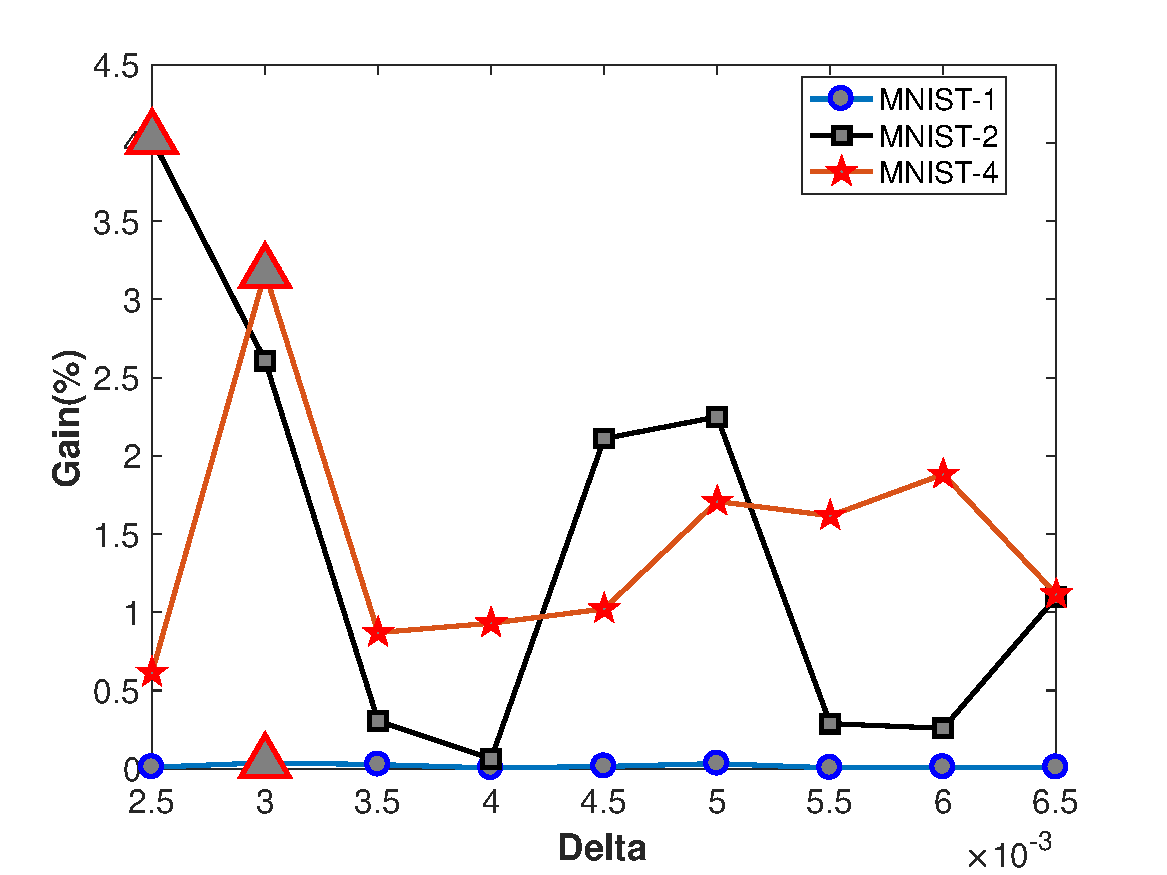
\includegraphics[keepaspectratio = True, scale = 0.31]{figures/MNIST_Delta}
		\centering
		\caption{MNIST}
		%    \vspace{2.0em}
	\end{subfigure}
	\begin{subfigure}[b]{.46\linewidth}
		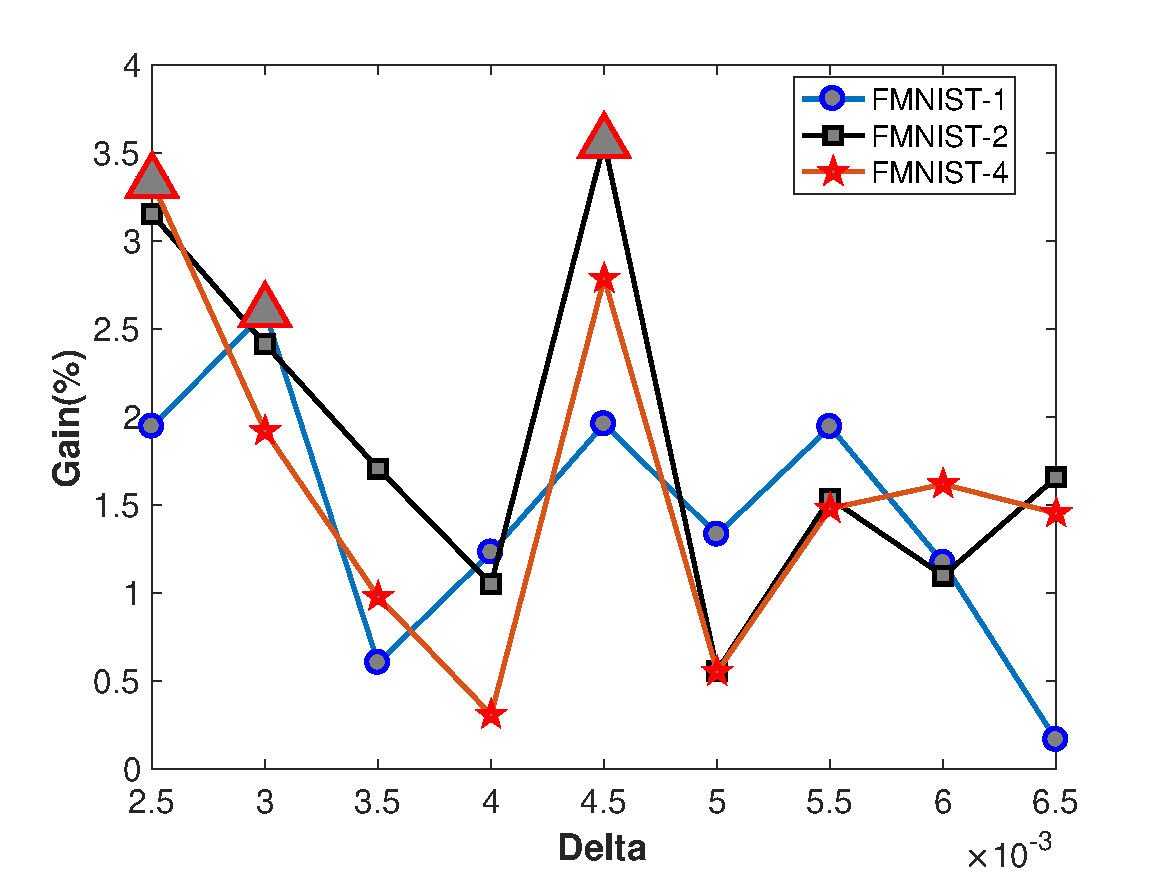
\includegraphics[keepaspectratio = True, scale = 0.31]{figures/FMNIST_Delta}
		\caption{F-MNIST}
		%    \vspace{2.0em}
	\end{subfigure}
	\caption{Experiment with varying $\delta$ and observe the gain of accuracy}
	\label{fig:delta}
\end{figure}
In our approach to identifying the optimum solution for the weight and bias discussed in Algorithm \ref{algo:asa}, the step size $\delta$ has not been decided. Instead of varying the $\delta$ while finding the appropriate value for weight and bias, we empirically evaluated our approach with different values of $\delta$ and identified the most suitable value. In this experiment, we have performed the 50 iterations for each choice of $\delta$ and pick the best gain to report in Figure \ref{fig:delta}. Also, to perform this experiment, we have not restricted our algorithm with a specific time and any desired gain. In Figure \ref{fig:delta}, we varied the value of $\delta$ from 0.002 to 0.0065 and observed the gain of accuracy. We performed this experiment for both MNIST and F-MNIST for all three different types of the model discussed before. We have denoted the highest gain for each model and dataset combination by an upward triangle. Our result suggests that five out of six evaluation conditions with $\delta$=0.0025 and $\delta$=0.003, the most gain has been achieved. For further evaluation, we have fixed the choice of the $\delta$ to either 0.0025 or 0.003.
\subsubsection{\textbf{RQ2: How effective is this approach?}}
\begin{figure}
	\begin{subfigure}[b]{.46\linewidth}{}
		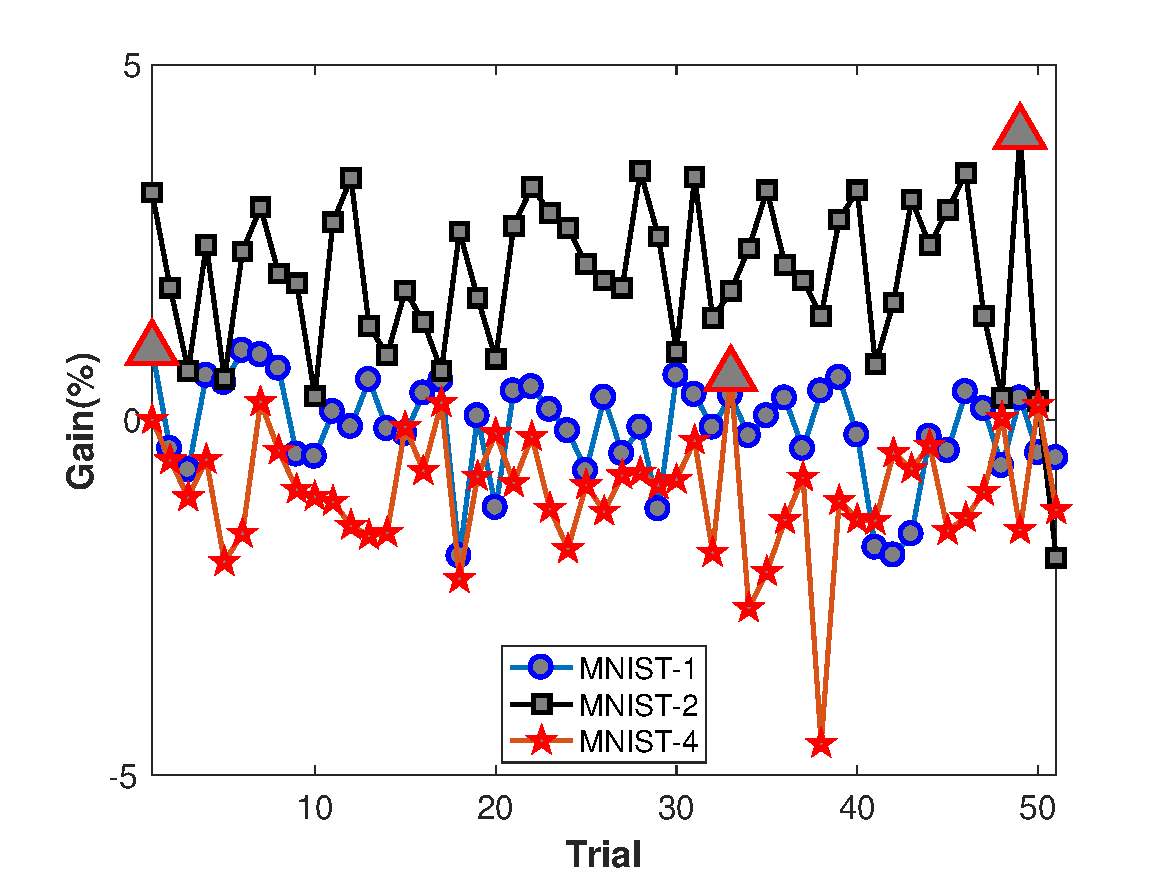
\includegraphics[keepaspectratio = True, scale = 0.31]{figures/MNIST_25}
		\centering
		\caption{MNIST}
	\end{subfigure}
	\begin{subfigure}[b]{.46\linewidth}
		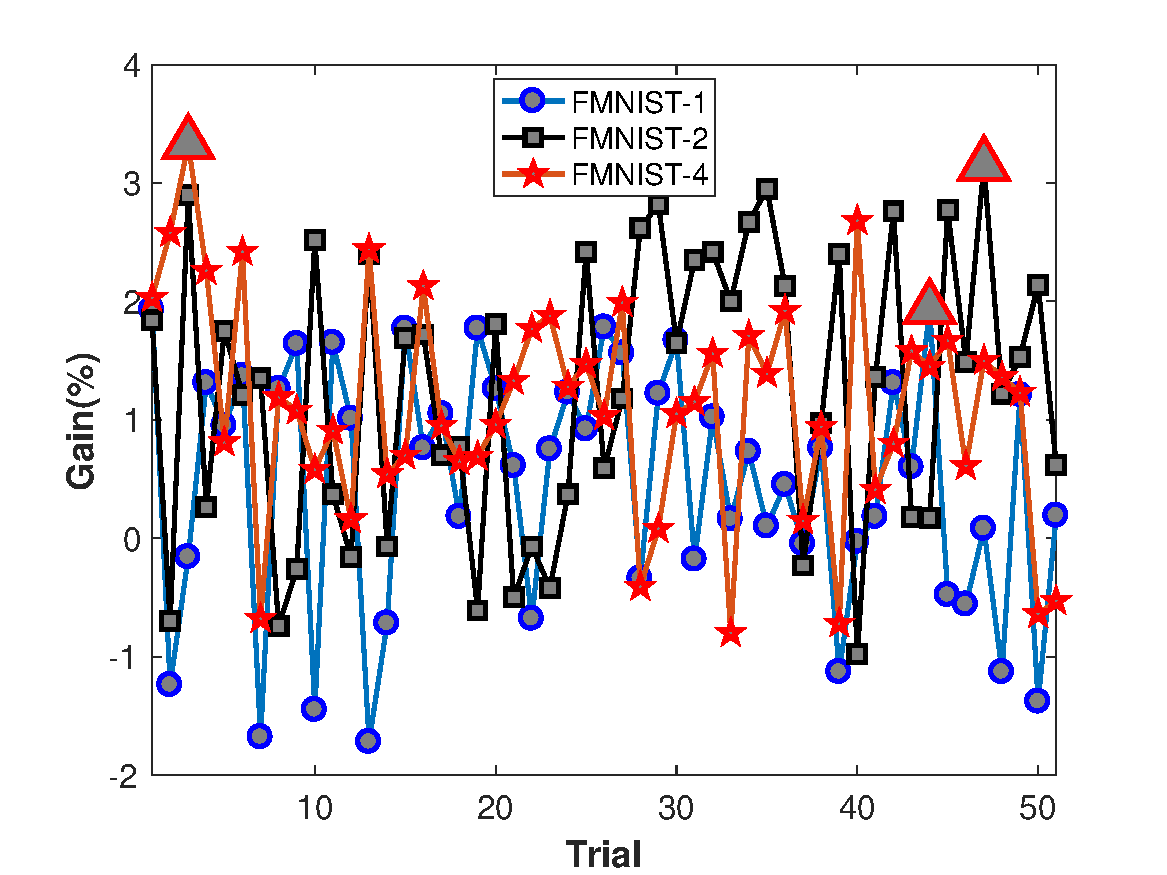
\includegraphics[keepaspectratio = True, scale = 0.31]{figures/FMNIST_25}
		\caption{F-MNIST}
	\end{subfigure}
	\caption{Trial with $\delta$=0.0025}
	\label{fig:trial1}
\end{figure}
\begin{figure}
	\begin{subfigure}[b]{.46\linewidth}{}
		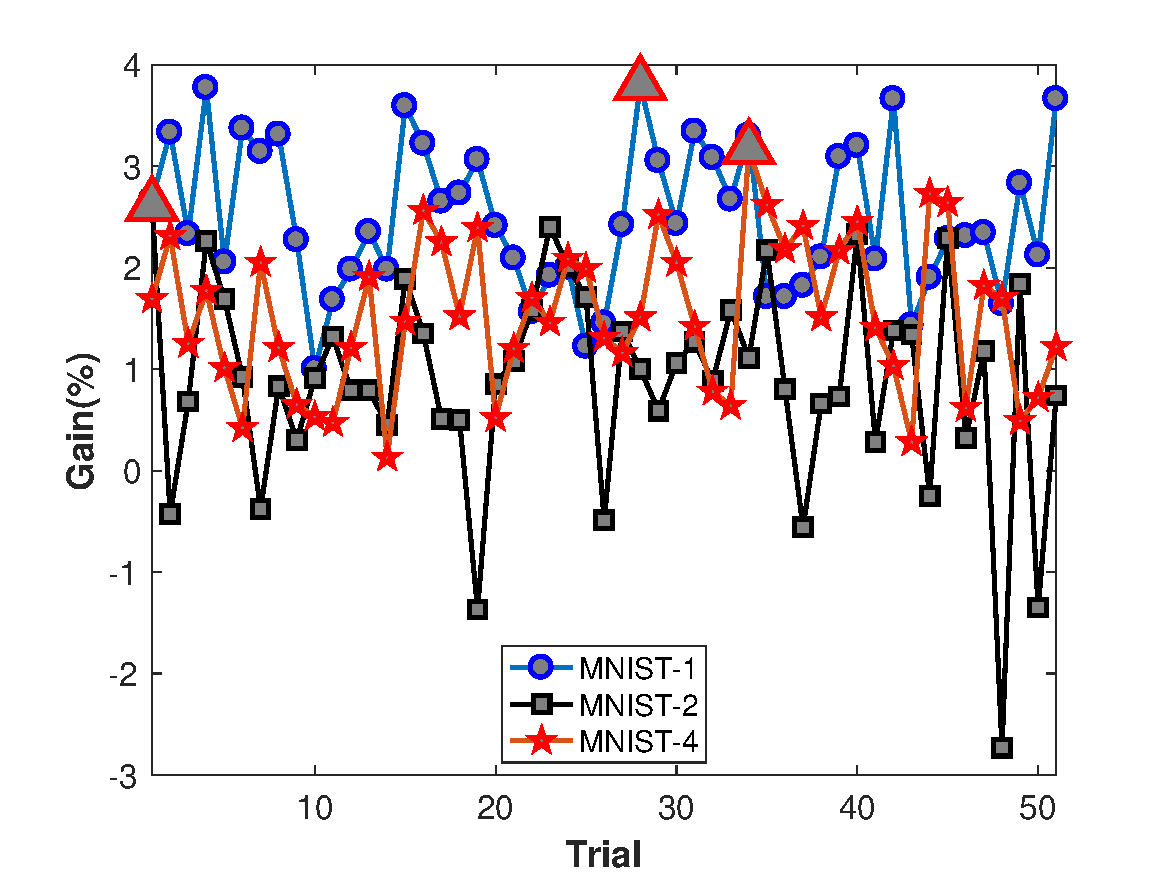
\includegraphics[keepaspectratio = True, scale = 0.31]{figures/MNIST_3}
		\centering
		\caption{MNIST}
		%\vspace{2.0em}
	\end{subfigure}
	\begin{subfigure}[b]{.46\linewidth}
		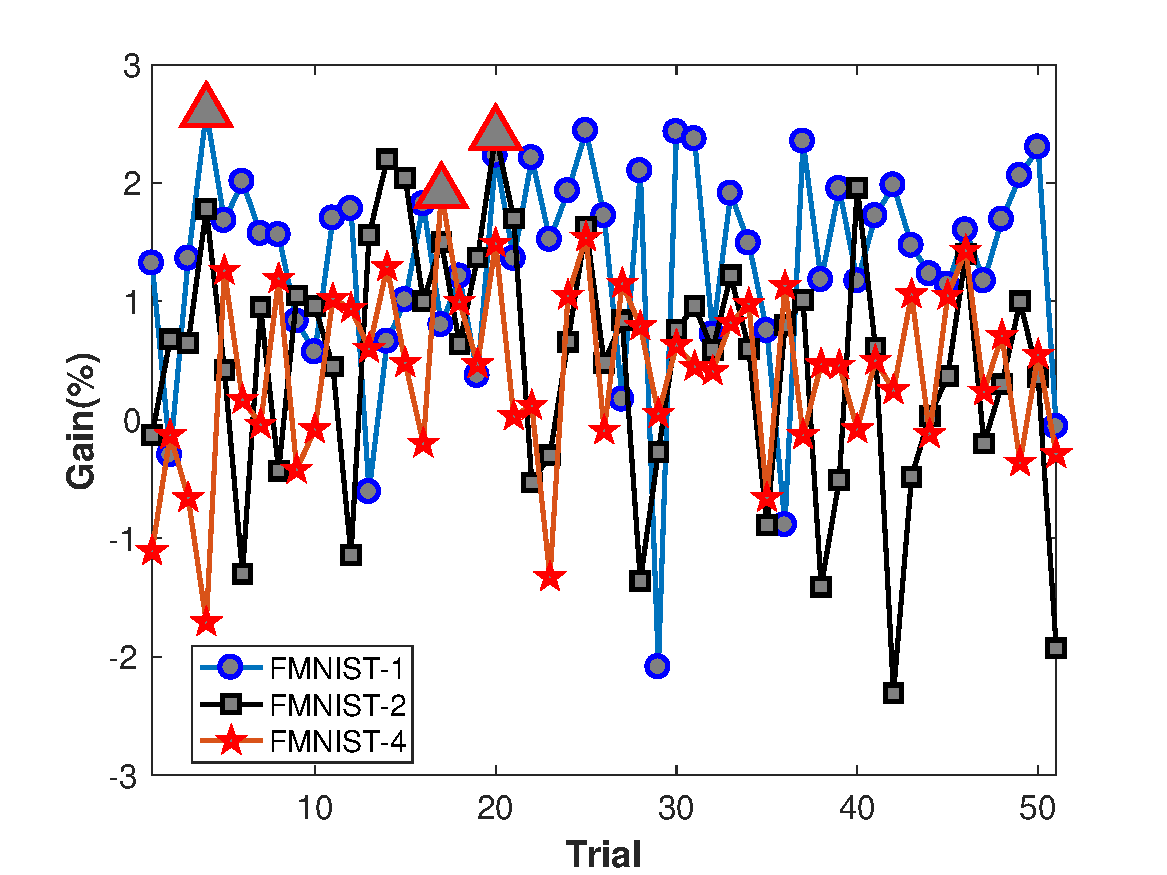
\includegraphics[keepaspectratio = True, scale = 0.31]{figures/FMNIST_3}
		\caption{F-MNIST}
		%\vspace{2.0em}
	\end{subfigure}
	\caption{Trial with $\delta$=0.003}
	\label{fig:trial2}
\end{figure}
To identify the gain achieved by our approach, we can utilize the same experimental setup discussed in the prior research question. We have found that our approach can increase the accuracy by 0.04\%, 4.02\%, and 3.17\% for MNIST dataset with model MNIST-1, MNIST-2, and MNIST-4 respectively. Whereas, for the F-MNIST dataset, our maximum gain achieved is 2.56\%, 3.55\%, and 3.33\% for FMNIST-1, FMNIST-2, and FMNIST-4 respectively. However, our approach takes a significant amount of time to identify the solution as for each $\delta$ value we have iterated our solution findings approach for 50 iterations that is equivalent to training the model 50 times. We have performed another set of experiments with the $\delta$ value found in our previous experiments. The primary reason to perform these new sets of the experiment to identify a set of values for iteration for which our approach performs best that can be helpful for end-users to restrict their choices. In the Figure \ref{fig:trial1}, we have performed the evaluation with the $\delta$=0.0025 and similarly, in Figure \ref{fig:trial2}, we have performed the experiments with $\delta$=0.003. We have evaluated all 6 combinations of models with 2 datasets. For each combination of model and dataset, we have denoted the maximum gain of accuracy by an upward triangle in the plots. From the experimental evaluation, we have found that there is no particular trend that the algorithm followed that can be used to restrict the value of the trials. The maximum gain of accuracy is almost distributed all over the places and with this message, we have not restricted our algorithm with any prior choice of the value for a number of allowable trials.

\subsubsection{\textbf{RQ3: How efficient is this approach?}}
We plan to measure the execution time for each iteration of evaluation and report the time needed to find the optimum solution for different $\delta$ and report the same.





